\documentclass[sigconf,natbib=false,10pt]{acmart}
\settopmatter{printacmref=false}
\setcopyright{none}
\renewcommand\footnotetextcopyrightpermission[1]{}

\acmConference[SOSP '24]{Workshop on Hot Topics in Operating Systems}{November
2024}{Austin, TX, USA}

%\begin{CCSXML}
%<ccs2012>
%   <concept>
%       <concept_id>10002978.10003029.10011703</concept_id>
%       <concept_desc>Security and privacy~Usability in security and privacy</concept_desc>
%       <concept_significance>300</concept_significance>
%       </concept>
%   <concept>
%       <concept_id>10002951.10002952.10003190</concept_id>
%       <concept_desc>Information systems~Database management system engines</concept_desc>
%%       <concept_significance>300</concept_significance>
%       </concept>
% </ccs2012>
%\end{CCSXML}

%\ccsdesc[300]{Security and privacy~Usability in security and privacy}
%\ccsdesc[300]{Information systems~Database management system engines}

% to be able to draw some self-contained figs
\usepackage{tikz}
\usepackage{amsmath}
\usepackage{hyperref}
\usepackage[normalem]{ulem}
\usepackage{listings}
\usepackage{xspace}
\usepackage{booktabs}
\usepackage{multirow}
\usepackage{wasysym}
\usepackage{caption}
\usepackage{subcaption}
\usepackage{enumitem}
\usepackage[utf8]{inputenc}
\usepackage[compact, small]{titlesec}

\captionsetup{labelfont=bf,textfont=rm,belowskip=-8pt,aboveskip=4pt}

% BibLaTeX for bibliography
\usepackage[
  backend=biber,
  style=numeric-comp,
  minalphanames=3,
  isbn=false,
  sortcites=true,
  sorting=anyt,
  abbreviate=false,
  url=false,
  doi=false,
  maxnames=99,
  minbibnames=3,
  maxbibnames=99]{biblatex}
\addbibresource{paper.bib}

\AtBeginBibliography{\small}
\setcounter{biburllcpenalty}{7000}
\setcounter{biburlucpenalty}{8000}

\newcommand\hmng[1]{\textcolor{blue!40!red}{[hmng: {#1}]}}
\newcommand\sysname{Cole}
\newcommand{\tabitem}{~~\llap{\textbullet}~~}
\newcommand{\eg}{{e.g.},\xspace}
\newcommand{\ie}{{i.e.},\xspace}

\newcommand{\one}{({\em i}\/)}
\newcommand{\two}{({\em ii}\/)}
\newcommand{\three}{({\em iii}\/)}
\newcommand{\four}{({\em iv}\/)}
\newcommand{\five}{({\em v}\/)}
\newcommand{\six}{({\em vi}\/)}



\lstdefinestyle{rust}{
    %backgroundcolor=\color{backcolour},
    commentstyle=\color{codegreen},
    keywordstyle=\color{codepurple},
    stringstyle=\color{blue},
    basicstyle=\ttfamily\scriptsize,
    breakatwhitespace=false,
    breaklines=true,
    captionpos=b,
    keepspaces=true,
    showspaces=false,
    showstringspaces=false,
    showtabs=false,
    tabsize=2
}
\lstset{style=rust}

%-------------------------------------------------------------------------------
\begin{document}
%-------------------------------------------------------------------------------

%don't want date printed
\date{}

%%
%% The "title" command has an optional parameter,
%% allowing the author to define a "short title" to be used in page headers.
% make title bold and 14 pt font (Latex default is non-bold, 16 pt)
\title{\sysname: know thine deadlines}

%%
%% The "author" command and its associated commands are used to define
%% the authors and their affiliations.
%% Of note is the shared affiliation of the first two authors, and the
%% "authornote" and "authornotemark" commands
%% used to denote shared contribution to the research.

% \author{
% {\rm Anonymous Authors}\\
% } % end author

\author{Hannah Gross}
\affiliation{%
 \institution{MIT}
 \state{Graduate Student}
  \country{}
}

\author{Frans Kaashoek}
\affiliation{%
 \institution{MIT}
 \state{}
  \country{}
}

\maketitle

%-------------------------------------------------------------------------------
\section{Introduction}
%-------------------------------------------------------------------------------

There is a fundamental mismatch between what developers care about (latencies)
and what they are required to give providers (resource reservations). Developers
use Service Level Objectives (SLOs) between teams and Service Level Agreements
(SLAs) towards customers, each of which represent promises about maximal latencies
of the API that team/company is in charge of (add citations). 

This mismatch is problematic on two levels: one is that the binary of
latency-critical and best effort is a false dichotomy, and the other is that
translating latencies into reservations is difficult. 

Imagine a web developer, whose website has four different types of work it has
to do: \\
(1) load static pages (eg the homepage) - short and very time ciritcal \\
(2) load dynamic pages (eg a users profile page) - slightly longer and less time
critcial \\
(3) foreground data processing (eg processing a user uploaded file of image) -
expected to take a bit, but should not run on forever \\
(4) background data processing (eg updating a data warehouse) - run overnight
and just needs to finish by morning.

The only real candidate for true best effort work is (4), and even that might be
difficult because it's a problem if it's not done by the time business picks up
the next day. For the other three, the translation to a reservation system then
happens offline, and requires the developer to make estimations about peak load
as well as how much they are willing to let latencies spike (for example, (3)
might be fine to run a bit slower when load is high but (1) should remain
completely impervious to load spikes). This estimation process also incentivizes
the developer to overestimate - low utilization is much less of a problem to them than
missing deadlines. 

This in turn poses a problem for providers, for whom high utilization means more
work they are able to run and thus more money. Bin-packing latency critical
work, as well as scheduling in best effort work opportunistically to use
resources guaranteed to latency critical jobs in time that they might not be
using it, is a hard problem that many systems work on.

What this work tries to do is avoid the problem alltogether. Rather than deal
with the lossy metric of reservations and the false binary of latency critcial
and best effort, this project attempts to create a spectrum of work, each job
being characterized by a deadline and a maximum compute time.

Work is submitted as a handler function, basically a binary. Attached is
metadata that includes the maximum execution time as well as a deadline. When a
request for this handler comes in, it is initially routed to the relevant shard
of a global scheduler. Depending on the amount of slack (difference between
deadline and max compute) the global scheduler will either immediately place the
job, or will probe a dynamic number of machines in order to find a good match.
Each machine has a dispatcher, which is in communication with a shard of the
global scheduler. The dispatcher accepts and runs work, as well as doing
back-of-the-envelope computation when probed about whether a new job would fit. 

The admission control is pessismistc, and assumes that every process will use
the maximum compute time. The dispatcher looks at the amount of slack each
process has (given the original slack and how much time it has already spent
waiting), and then judges whether a new process would still allow it to meet all
the max compute guarantees. Once admitted to a machine, work is run using an
approximation of Earliest Deadline First (EDF) scheduling. This is acheived via
a slight abuse of linux' new scheduling algorithm, Earliest Eligible Virtual
Deadline First (EEVDF), originally proposed in the 90s and recently integrated
as linux' scheduling algorithm for the normal scheduling class. It also required
editing linux in a small way to make its behavior closer to the original paper
(from which the linux implementation diverges in meaningful ways).


%-------------------------------------------------------------------------------
\section{Design}
%-------------------------------------------------------------------------------

\begin{figure}[t!]
    \centering
    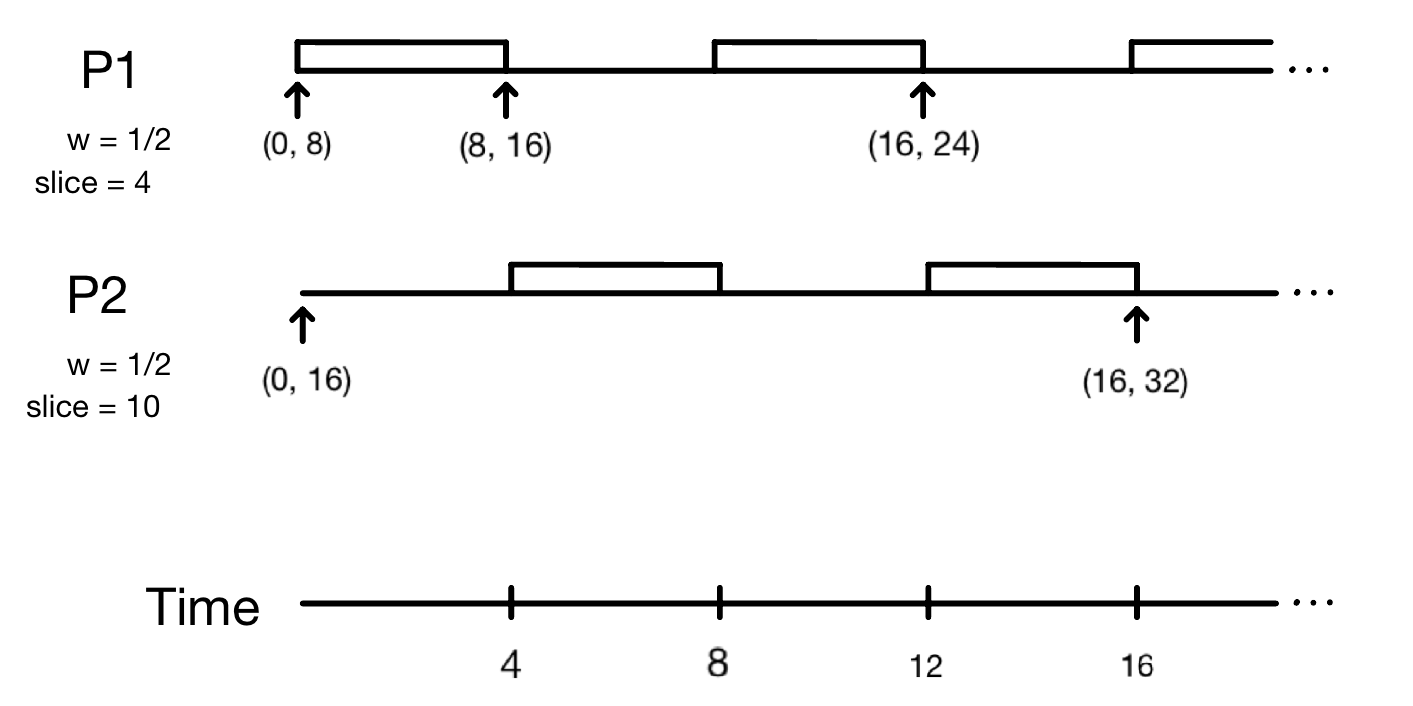
\includegraphics[height=1.5in]{img/eevdf.png}
    \caption{An example EEVDF timeline. Arrows represent requests, denoted with time eligible and deadline, 
        and boxes showing which process is chosen to run. }
    \label{eevdf}
\end{figure}

\begin{figure*}[h!]
    \centering
    \begin{subfigure}[t]{0.5\textwidth}
        \centering
        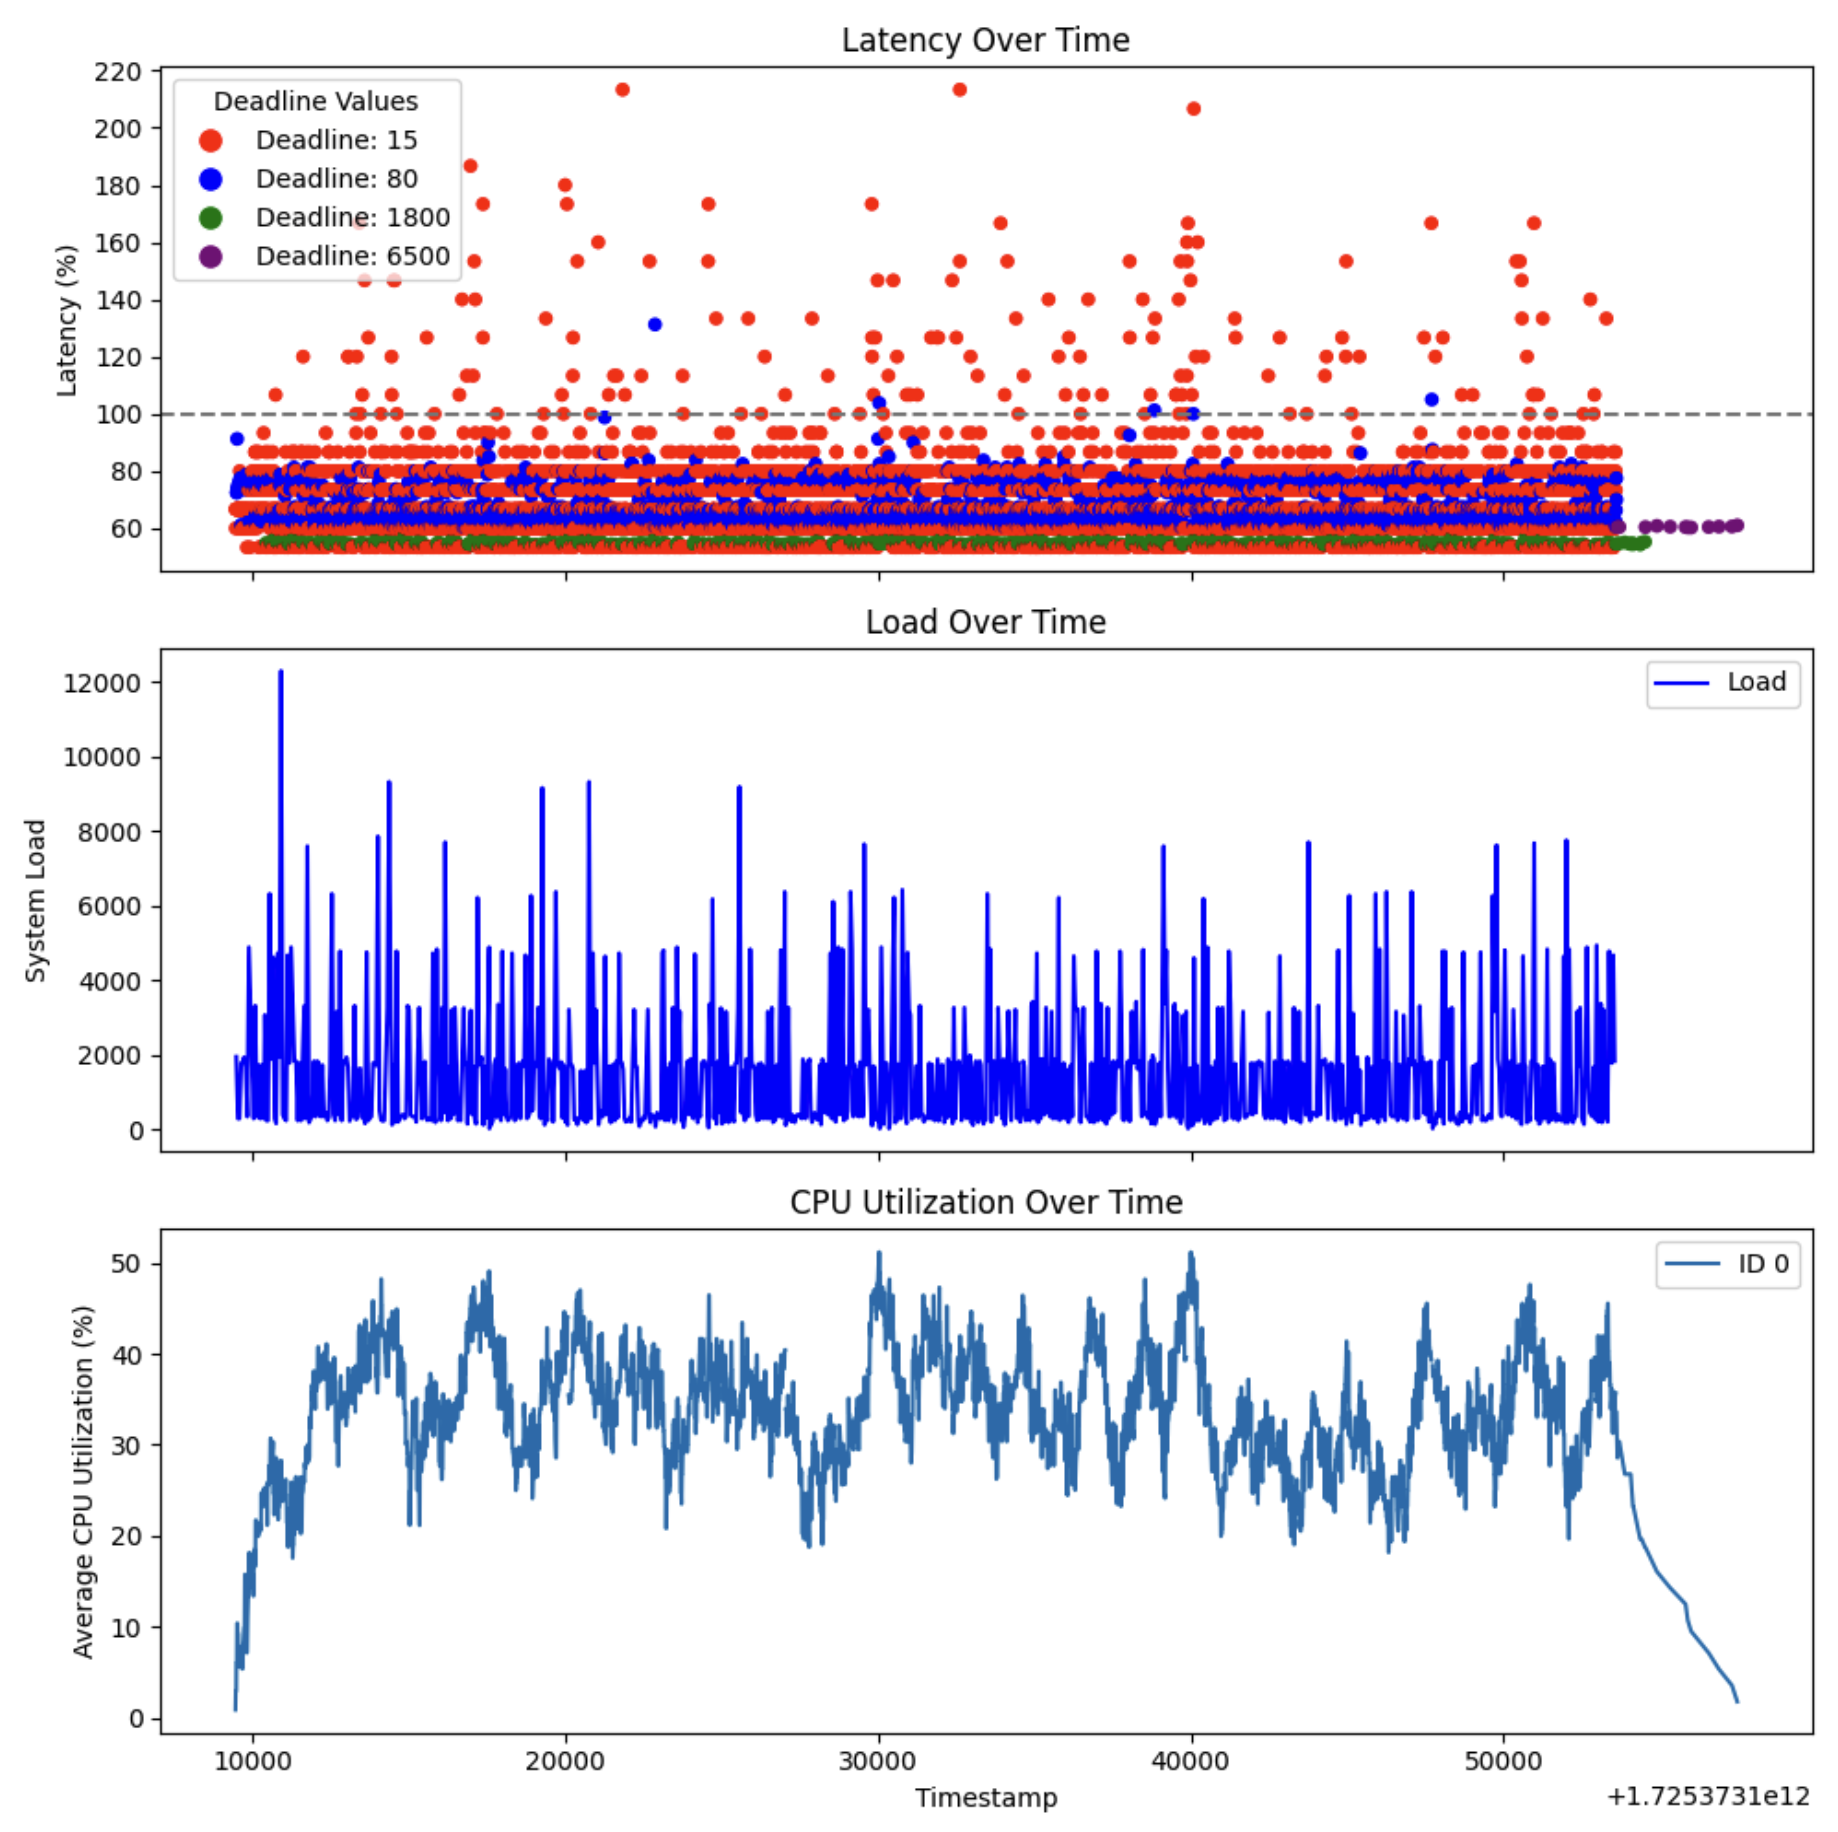
\includegraphics[height=2in]{img/old_lnx__2ms_wait__10K_iter.png}
        \caption{Latency and utilization in original linux}
    \end{subfigure}%
    \hfill
    \begin{subfigure}[t]{0.5\textwidth}
        \centering
        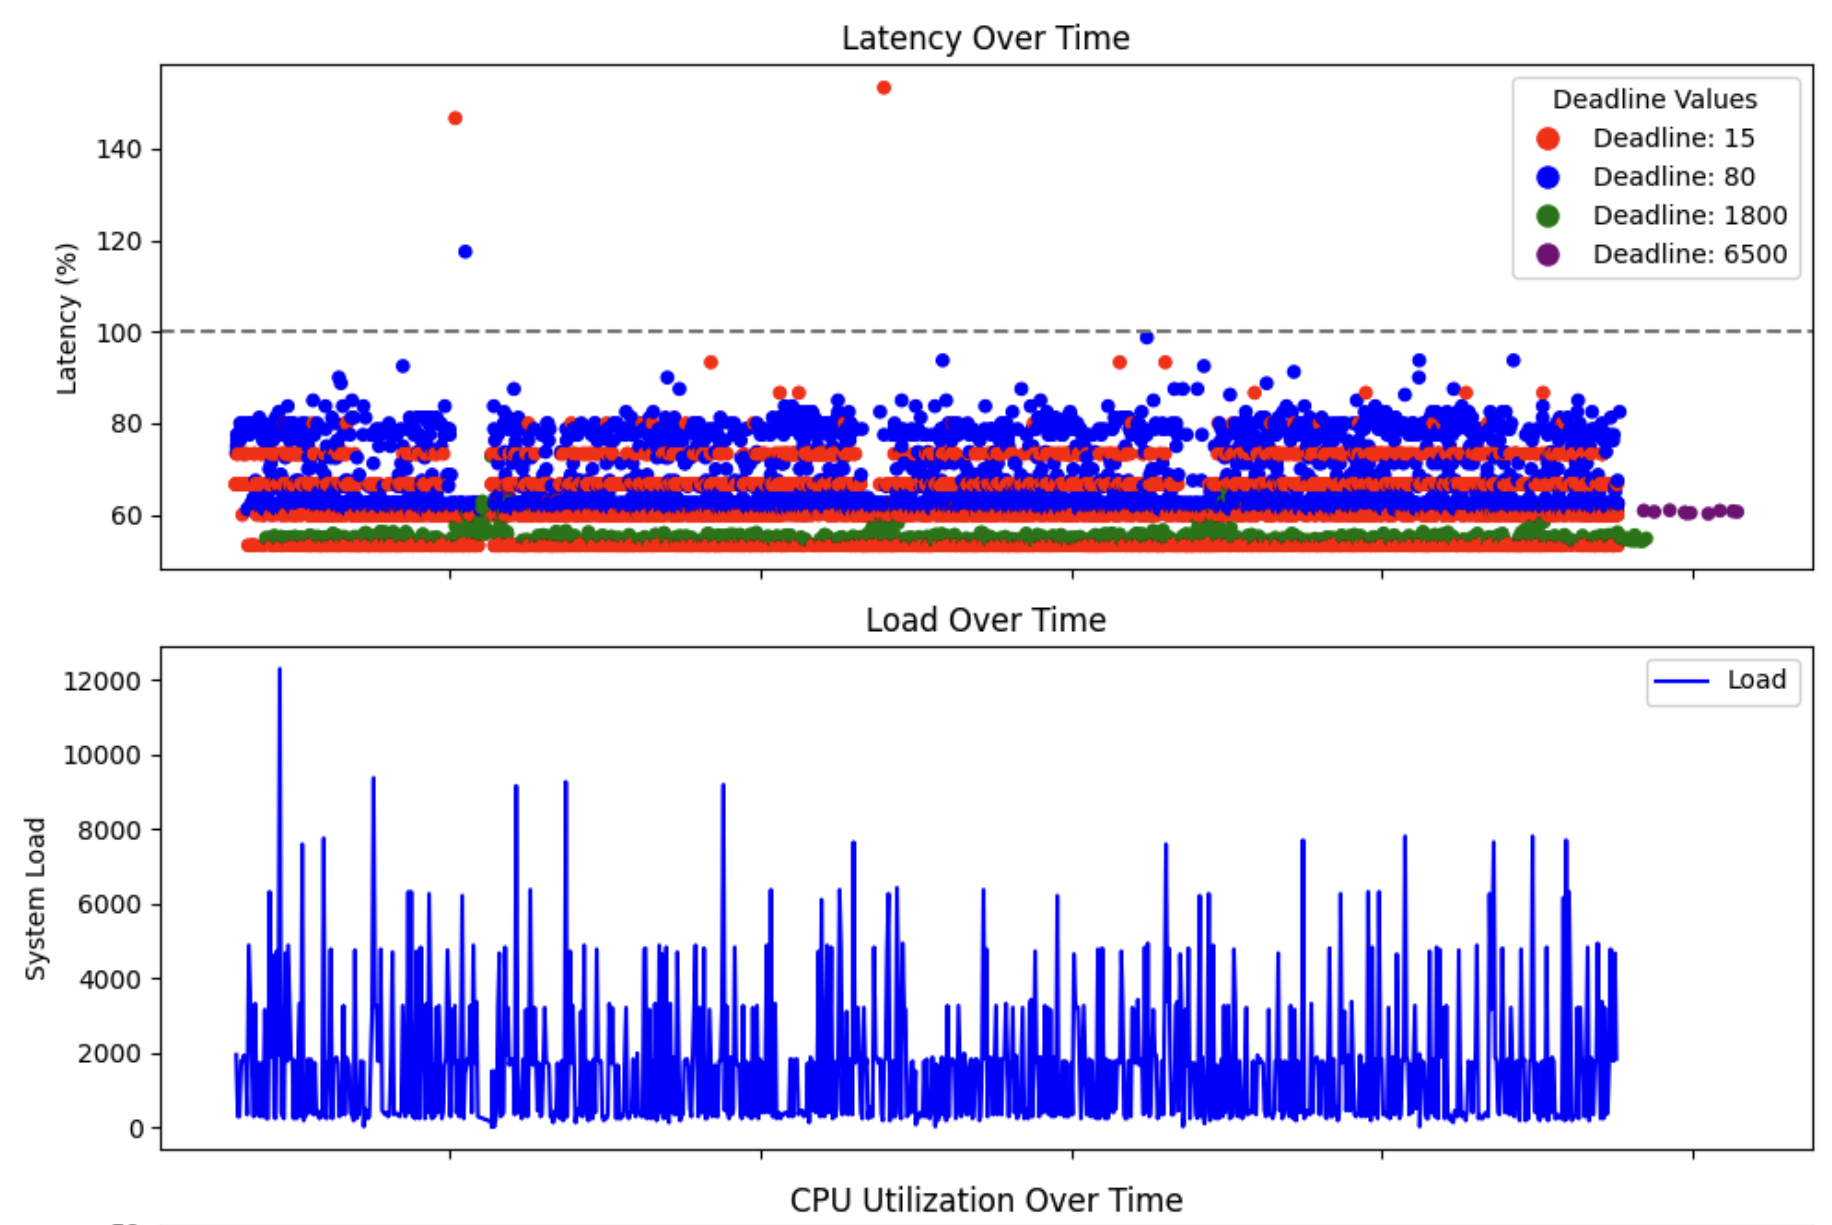
\includegraphics[height=2in]{img/new_lnx__2ms_wait__10K_iter.png}
        \caption{Latency and utilization in modified linux}
        \label{fig:graph:new}
    \end{subfigure}
    \vspace{10pt}
    \caption{Results of running the same workload on (a) unmodified and (b) modified linux.}
    \label{fig:graph}
\end{figure*}

Developers submit jobs, attached with the maximum execution time as well as a
deadline. 

When a job is run, it is initially routed to the relevant shard of the
\textit{global scheduler} \ref{DGS}, which then forwards the job to a chosen
single machine \ref{SM}. 


\subsection*{Distributed Global Scheduler}
\label{DGS}

Each global scheduler shard has a set of machines that it can run jobs on. The
goal of the global scheduler is to keep load as evenly distributed among these
machines as possible, in the sense that each machine has a maximally
heterogenous set of deadlines and computes. This allows processes with more
\textit{slack} (difference between deadline and max compute) to fill in gaps
where shorter processes might have finished earlier than expected (similarly to
how best effort work now opportunistically uses resources not currently used by
latency critical tasks).

Depending on the amount of slack the global scheduler will either immediately
place the job, or will probe a dynamic number of machines in order to find a
good match.


\subsection*{Single machine}
\label{SM}

On the individual machines, the goal is to to meet all the deadlines of the work
assigned to the machine. This has two parts: one is a dispatcher thread, which
handles communication with its global scheduler shard and does admission
control; and the other is a local scheduler that prioritizes work by deadline.

Admission control is pessismistc, and assumes that every process will use the
maximum compute time. The dispatcher looks at the amount of slack each process
has (given the original slack and how much time it has already spent waiting),
and then judges whether a new process would still allow the machine to meet all
the maximum compute guarantees.


The local scheduler approximates Earliest Deadline First (EDF) scheduling.
\sysname{} acheives EDF scheduling by using EEVDF - originally proposed in the 90s
and recently integrated in linux - at one extreme.

% have a figure with two processes making requests and getting time?

In EEVDF, processes make requests for resources, and each request is assigned an
eligible time and a deadline. At every scheduling point, of the eligible
processes the one with the earliest deadline is chosen to run next. Eligible
times and deadlines are in virtual time, which allows for oversubscription. 

Processes need to be able to be ineligible in order to maintain fairness. If a
process ran for the last tick and completed its latest request, its next
eligible time will be set to be in the future (a weighted estimation of by when
it should have gotten the time it just did, based on its weight as well the the
total system load). This protects against starvation of processes with longer
deadlines.

If jobs make requests often and for small time increments, this policy is
similar to PS - each process runs for a scheduling quanta before becoming
ineligible. However, on the other extreme you get behavior closer to EDF - if
jobs only ever make one request for all the resources that they think they will
need, then the requests never reset and all processes are always elgibible,
leading the EDF choice to be among all processes.

And creating this edge condiiton is what the dispatcher does - when it spawns a
process for a new job, it sets the requested timeslice of that job to be the
jobs maximum compute. 


%-------------------------------------------------------------------------------
\section{Current State}
%-------------------------------------------------------------------------------

Implementing this design required changing Linux's EEVDF implementation. Linux's
EEVDF scheduler has a strong tenant of avoiding unfairness, and as a result
implements eligibility solely as a function of how much time a process had
gotten compared to other processes. This means that (assuming equally weighted
processes), after a tick of running, a process becomes ineligible, because it
got more time that it should have (in an ideal system the tick would have been
shared equally among all processes).

In \sysname, however, being able to be unfair for long periods of time is key:
jobs with short deadlines need to get absolute priority over jobs that have
later deadlines. To achieve this goal we had to modify Linux's EEVDF
implementation, to include the notion of request-based eligibility.

We developed a prototype application that follows the scheme of the website:
four different types of jobs, with deadlines ranging from 15ms to 6s, and
maximum computes from 12ms to 4s. Figure~\ref{fig:graph} shows the results on a
single machine, with and without the change to Linux. 

Overall the graph shows success: being temporarily unfair to longer processes
that had a large amount of slack allowed the shorter processes with less slack
to consistently complete on time.
\section{Related Work}

There is a large body of work that focuses on removing the need for
reservations by creating elastic reservations that automatically scale up and
down with load~\cite*{kubernetes, snowflake}. These systems generally
operate on a much larger timescale (control loops on the order of many
seconds~\cite{kubernetestime}), and still work within the best effort
- latency critical binary. 

There are systems that focus on increasing utilization via much more
fine-grained preemption behavior~\cite*{caladan, shinjuku}. These require
building a kernel-bypass scheduler. 

Other work does operate on the basis of deadlines, but take different approach
to realizing those deadlines. Some try to formally pre-compute compute time to
make guarantees~\cite{jockey}, while others use the deadline to generate a
reservation~\cite*{rayon}. Morpheus~\cite*{morpheus} targets jobs with
invocation frequencies of around a day, and infers the deadline from historic
data, automatically generating recurring reservations.



%-------------------------------------------------------------------------------
% \bibliography{paper.bib}
\printbibliography

%%%%%%%%%%%%%%%%%%%%%%%%%%%%%%%%%%%%%%%%%%%%%%%%%%%%%%%%%%%%%%%%%%%%%%%%%%%%%%%%
\end{document}
%%%%%%%%%%%%%%%%%%%%%%%%%%%%%%%%%%%%%%%%%%%%%%%%%%%%%%%%%%%%%%%%%%%%%%%%%%%%%%%%

%%  LocalWords:  endnotes includegraphics fread ptr nobj noindent
%%  LocalWords:  pdflatex acks
